\documentclass[11pt,a4paper]{article}

\usepackage[T1]{fontenc}
\usepackage[utf8]{inputenc}
\usepackage[frenchb]{babel}

\usepackage{fancyhdr} % headers
\usepackage[usenames,dvipsnames]{color} % colors
\usepackage{graphicx} % images
\usepackage{listings} % source code
\usepackage{titling} % meta-infos
\usepackage{courier} % courier font
\usepackage{fullpage} % full page layout
\usepackage{titlesec} % title customization
\usepackage{parskip} % paragraphs spacing
\usepackage{amsmath}
\usepackage{tikz}
\usepackage{siunitx}
%\usepackage{showframe} % layout debug

\usepackage{float}
\restylefloat{figure}

\topmargin -10mm
\headsep 5mm
\headheight 10mm

\linespread{1.1}
\renewcommand{\arraystretch}{1.3}

\setlength\parindent{0pt}
\setlength{\unitlength}{1cm}
\setlength{\droptitle}{-1.6cm}

\pagestyle{fancy}
\fancyhf{}
\cfoot{\thepage}

\def \doccourse { TIB1-B }
\def \doctitle {Labo : Structure d'Internet}
\author{Bastien Clément \and Christophe Peretti}

\renewcommand{\thesection}{Objectif \arabic{section} :}
\renewcommand{\thesubsection}{\arabic{section}.\arabic{subsection}}

\rhead{\theauthor \\ \today}
\lhead{\doccourse \\ \doctitle }
\title{{\normalsize \doccourse} \\ \doctitle }

\begin{document}

\maketitle
\vspace{1em}

\section{Outils}

L'objectif de cette première partie de laboratoire est de se familiariser avec des outils permettant la découverte de la structure d'Internet (\texttt{tracepath} et \texttt{traceroute}, \texttt{nslookup}) et interpréter les résultats obtenus avec ces outils.

\subsection{Commandes \texttt{traceroute} et \texttt{tracepath}}

Ces deux programme sont pratiquement équivalents. La page \texttt{man} de \texttt{tracepath} le décrit même comme \textit{traceroute without fancy options}. Ils permettent tout deux de tracer l'itinéraire emprunté par un paquet IP pour rejoindre une destination spécifique.

Ces programmes utilisent le champs TTL (\textit{Time-To-Live}) des paquets IP qui spécifie après combien d'intermédiaire le paquet doit être considéré invalide et détruit même s'il n'a pas encore atteint sa destination. Un message informant notre machine de l'erreur est alors envoyé par la machine ayant détruit le paquet.

Tous les routeurs ne respectent pas obligatoirement ce mécanisme. Il est donc parfois possible qu'aucun message d'erreur ne soit reçu permettant d'identifier l'intermédiaire suivant.

\subsection{Interprétation des résultats}

\begin{lstlisting}[basicstyle=\small,frame=single]
traceroute to w3.hes-so.ch (84.16.89.24), 64 hops max, 52 byte packets
 1  swiyv2.switch.ch (193.134.216.13)  26.850 ms  26.314 ms  24.538 ms
...
 5  cixp.infomaniak.ch (192.65.185.140)  25.862 ms  26.062 ms  28.890 ms
...
 8  www.hes-so.ch (84.16.89.24)  25.910 ms  26.285 ms  26.094 ms
\end{lstlisting}

Pour chaque étape, trois paquets de mesure sont envoyés. Les colonnes indiquent successivement:

\begin{enumerate}
	\item Le nombre de nœuds parcourus jusqu'à la destruction du paquet
	\item Les adresses DNS et IP de la machine atteinte
	\item Le temps d'\textit{aller-retour} des trois paquets
\end{enumerate}

\section{Structure d'Internet en Suisse}

L'objectif de cette partie est d'utiliser les outils vus précédemment pour découvrir la structure des réseaux composant Internet en Suisse et dessiner un plan des interconnexions observées.

\subsection{Carte des réseaux interconnectés}

\begin{center}
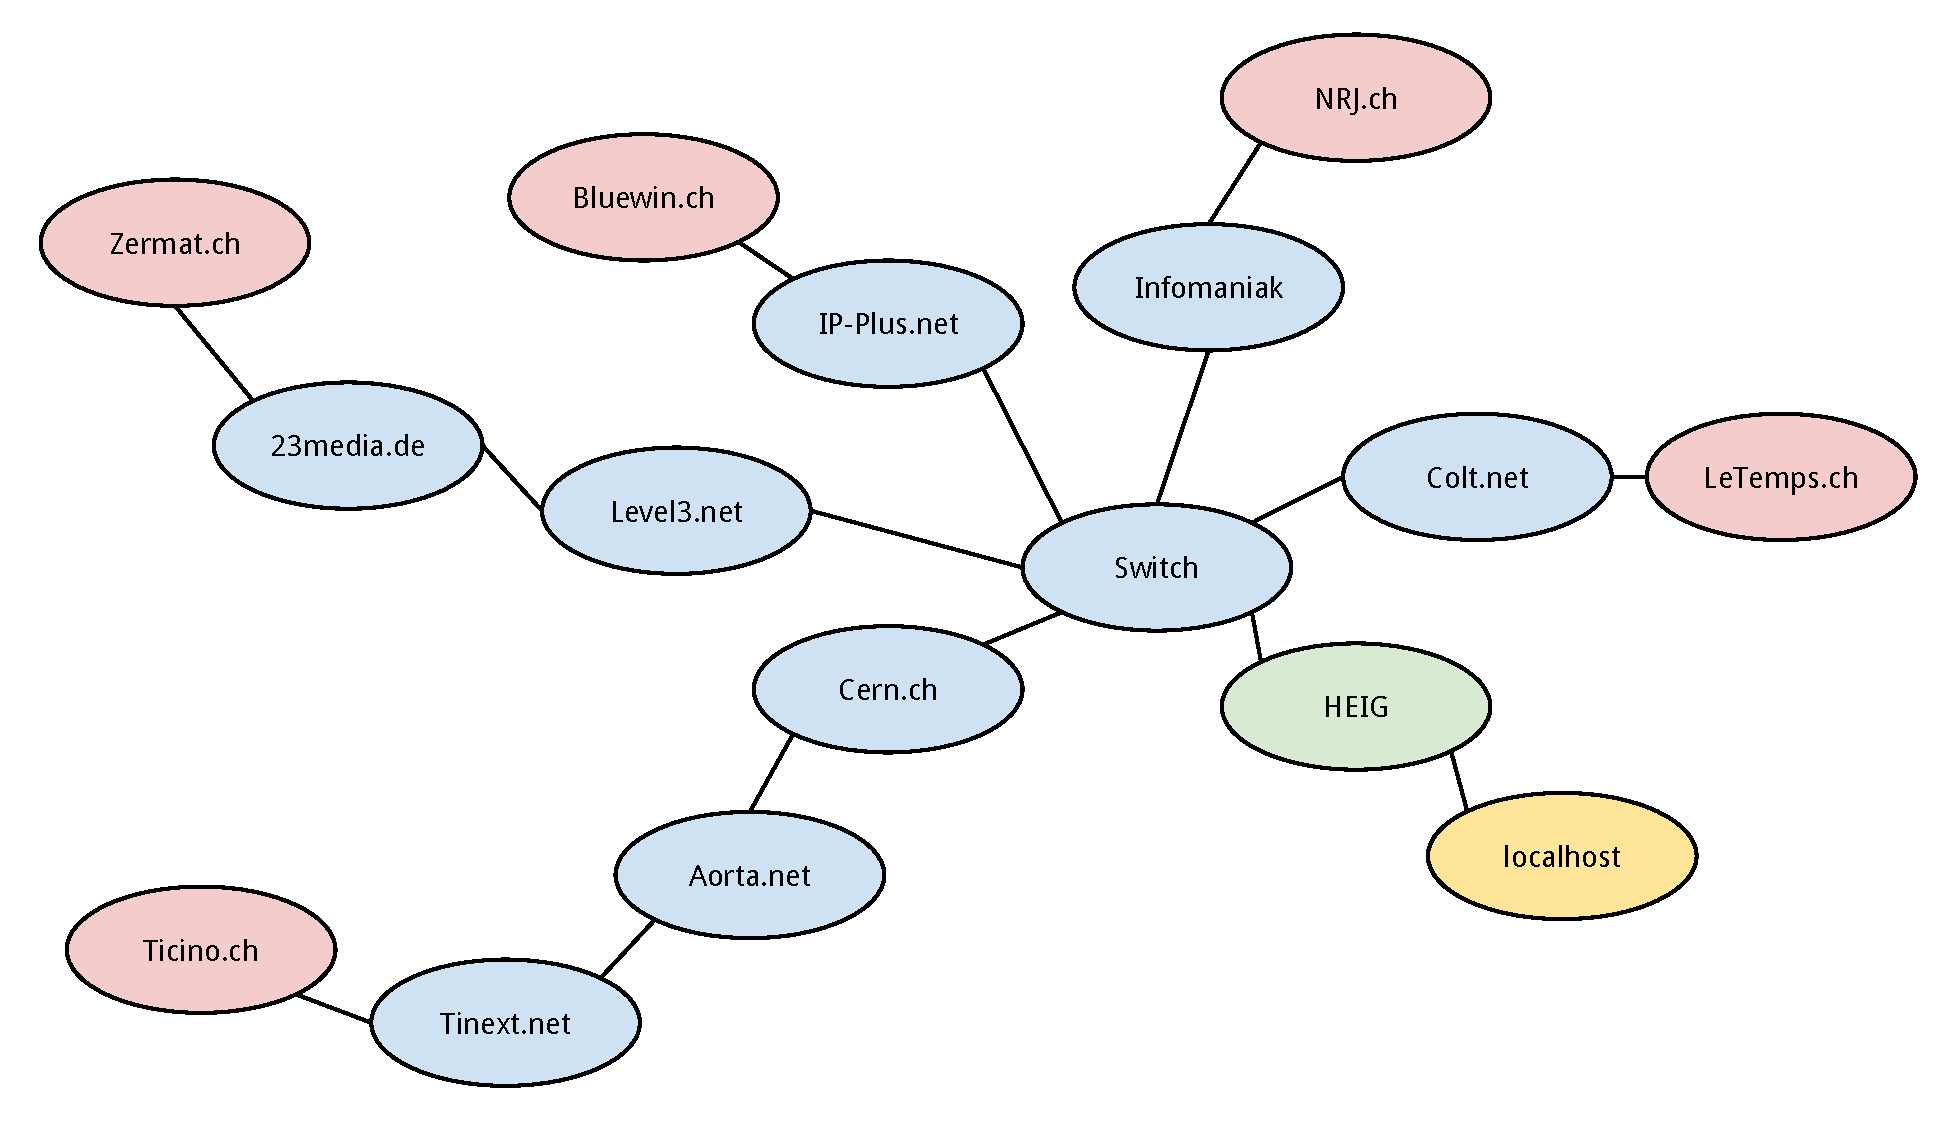
\includegraphics[width=15cm]{img_suisse}
\end{center}

Le fournisseur d'accès Internet de la HEIG-VD est Switch. Sans surprise donc, pour chaque destination que nous avons testé, les paquets passent premièrement par Switch avant d'être routés plus loin dans le réseau.

\subsection{Description des réseaux}

Nous observons ici quelques noms bien connus tel que \textit{Infomaniak} qui est un des plus important hébergeur suisse, \textit{IP-Plus} qui correspond à la branche de services professionnels de \textit{Swisscom} ainsi que \textit{Level3} qui occupe une place importante dans les réseaux internationaux européens, comme nous pourrons le voir dans la prochaine partie.

\section{Structure d'Internet globale}

\subsection{Carte}

\begin{center}
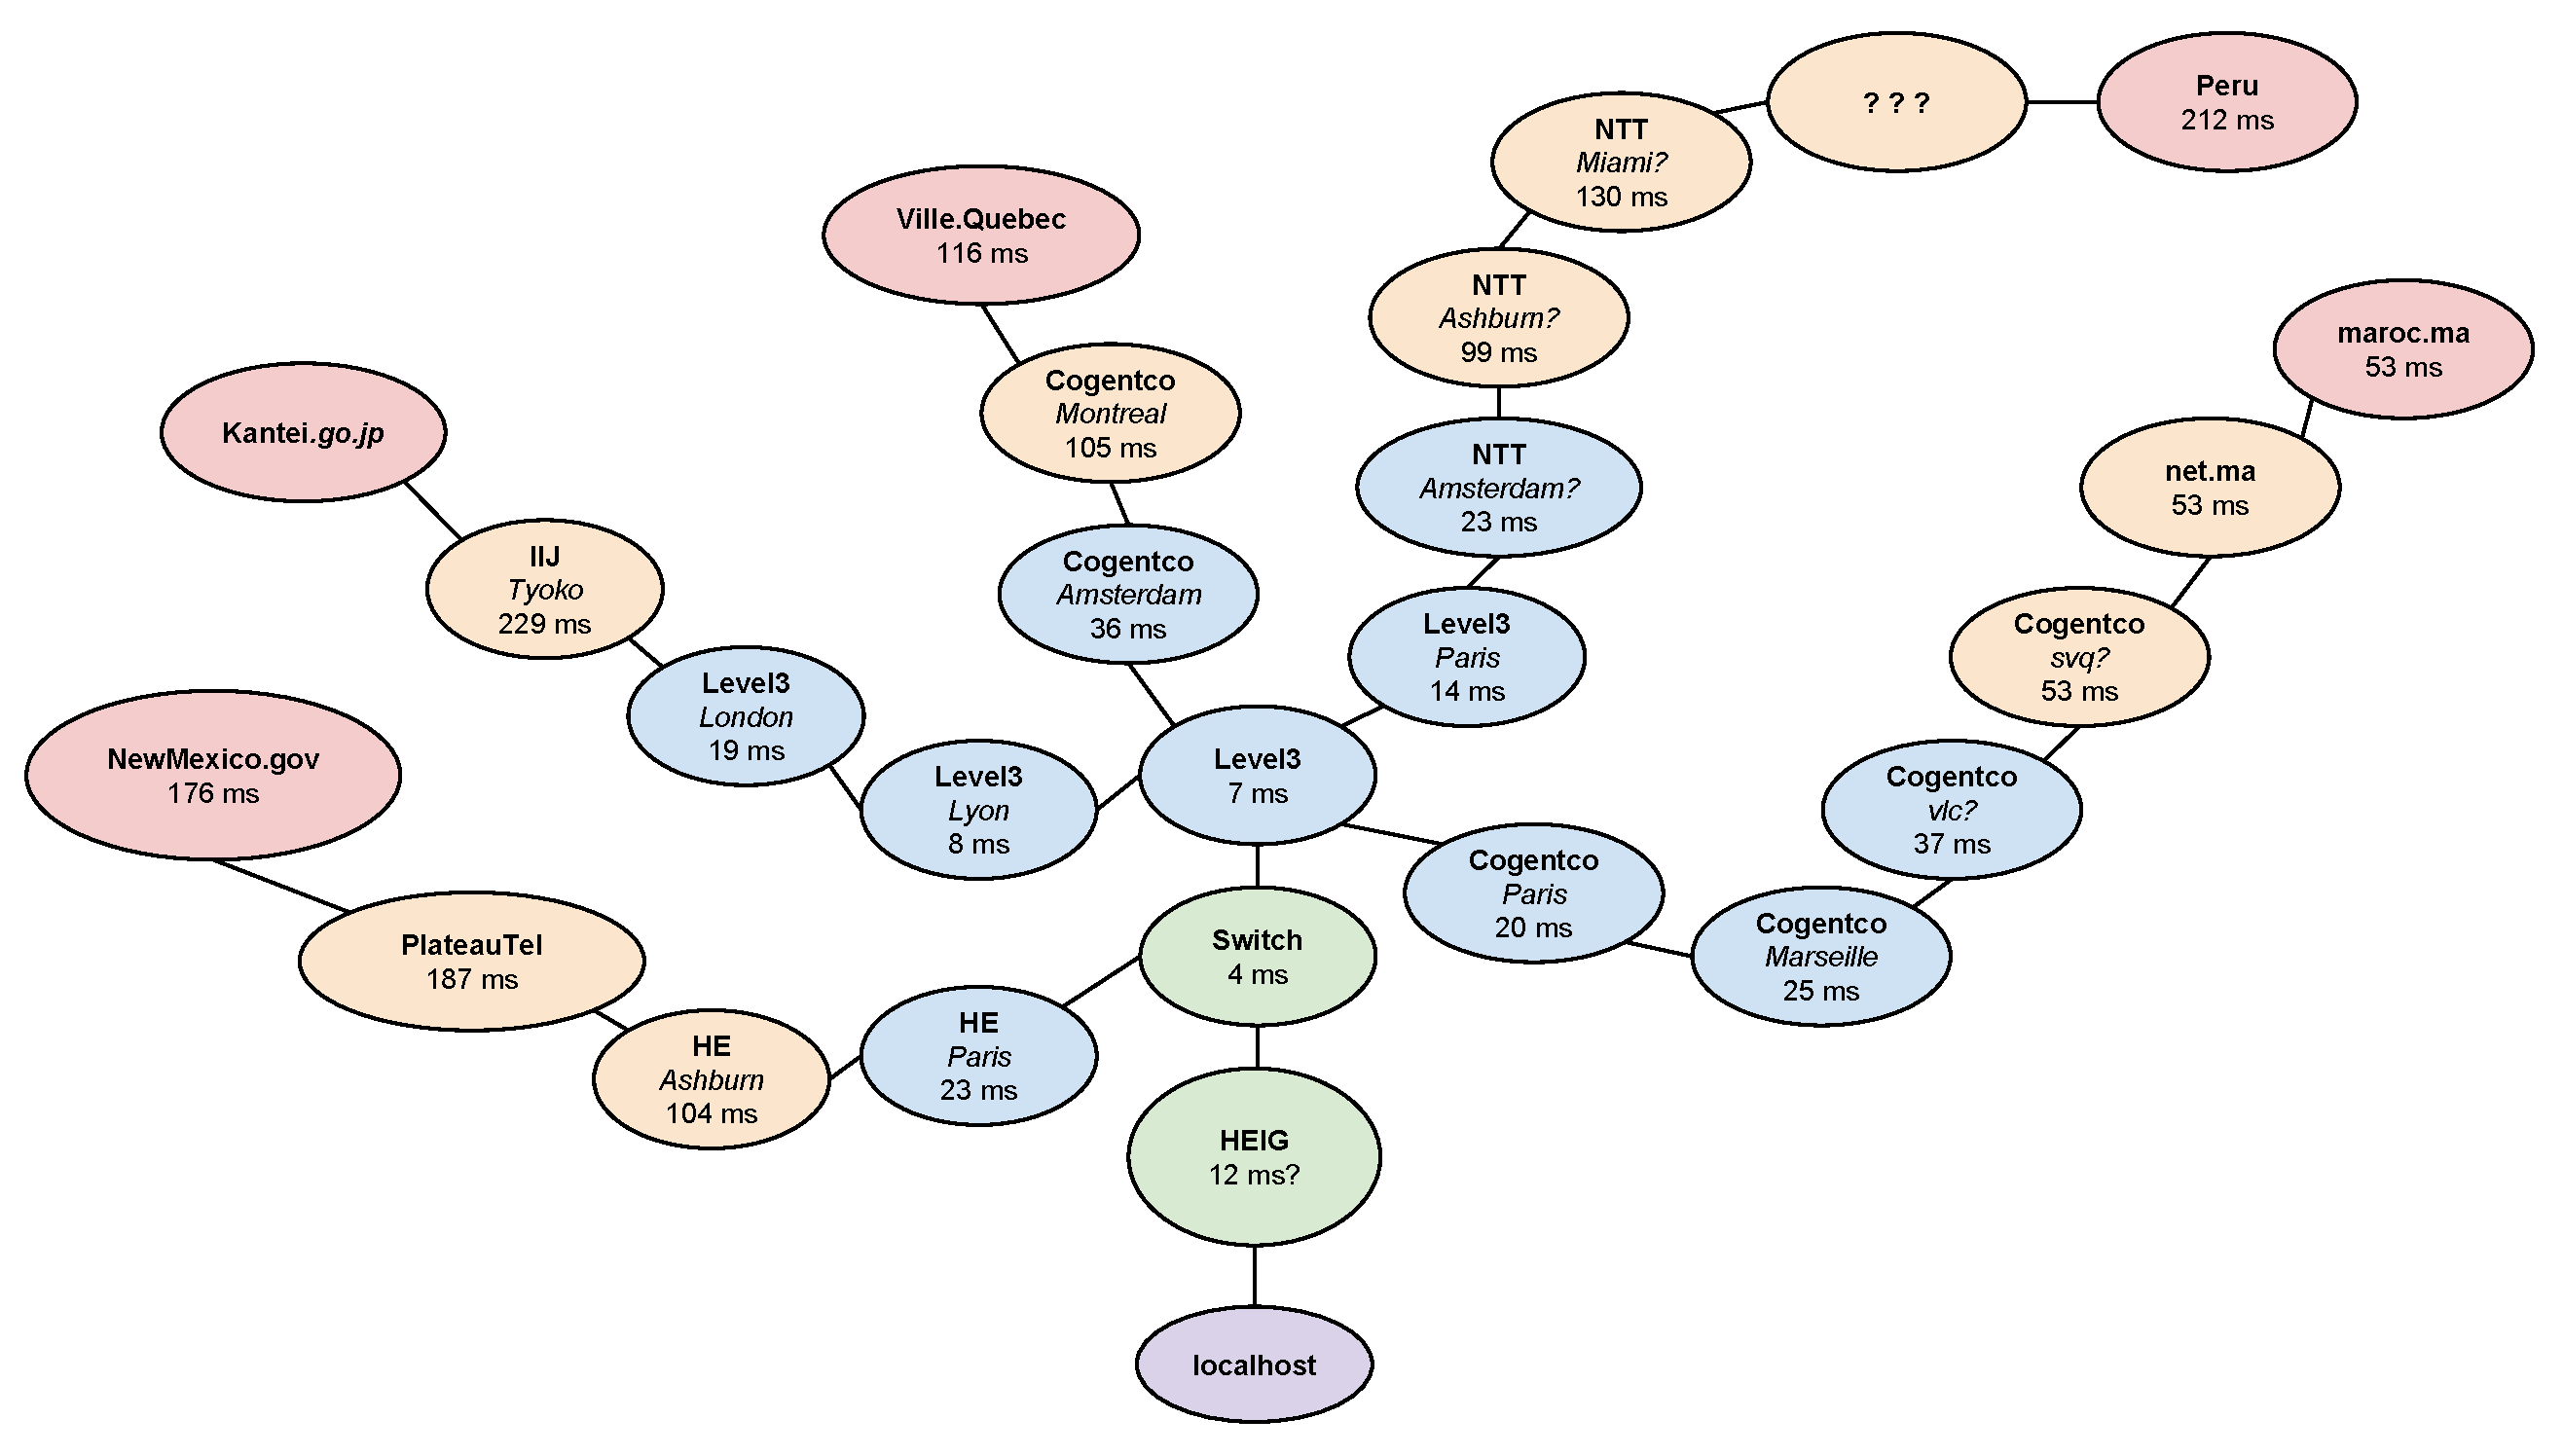
\includegraphics[width=15cm]{img_world}
\end{center}

Bla bla bla !

\section*{Auto-évaluation}

Nous considérons avoir atteint les objectifs de ce laboratoire.

\end{document}